\chapter{КОМПОНЕНТНАЯ БАЗА}
\section{Введение}
\textit{Дописать с соответствием с ТЗ в 1.4}

В выборе компонентной базы мы будем руководствоваться следующими параметрами:
\begin{itemize}
\item простота интеграции;
\item дешевизна;
\item эргономичность.
\end{itemize}

\section{Контроллер}
Если выбирать один контроллер, то он должен поддерживать инитерфейс USB, SPI, иметь достаточное количество цифровых и аналоговых входов/выходов(в соответствии с предведущей главой см.рис.\ref{fig:graf:AppShcSys} на страницена странице \pageref{fig:graf:AppShcSys}), а кроме частота тактирования должна быть достаточно, чтобы поддерживать VGA интерфейс. На рынке есть процессор Atmel SAM3X8E ARM Cortex-M3 на его базе плата DUE V1.6 от Elecfreaks(см. рис.\ref{fig:DueBoard}) с следующими характеристиками см. табл.\ref{tab:DueBoard}\cite{s_1}.
\begin{figure}[ht]
	\centering
     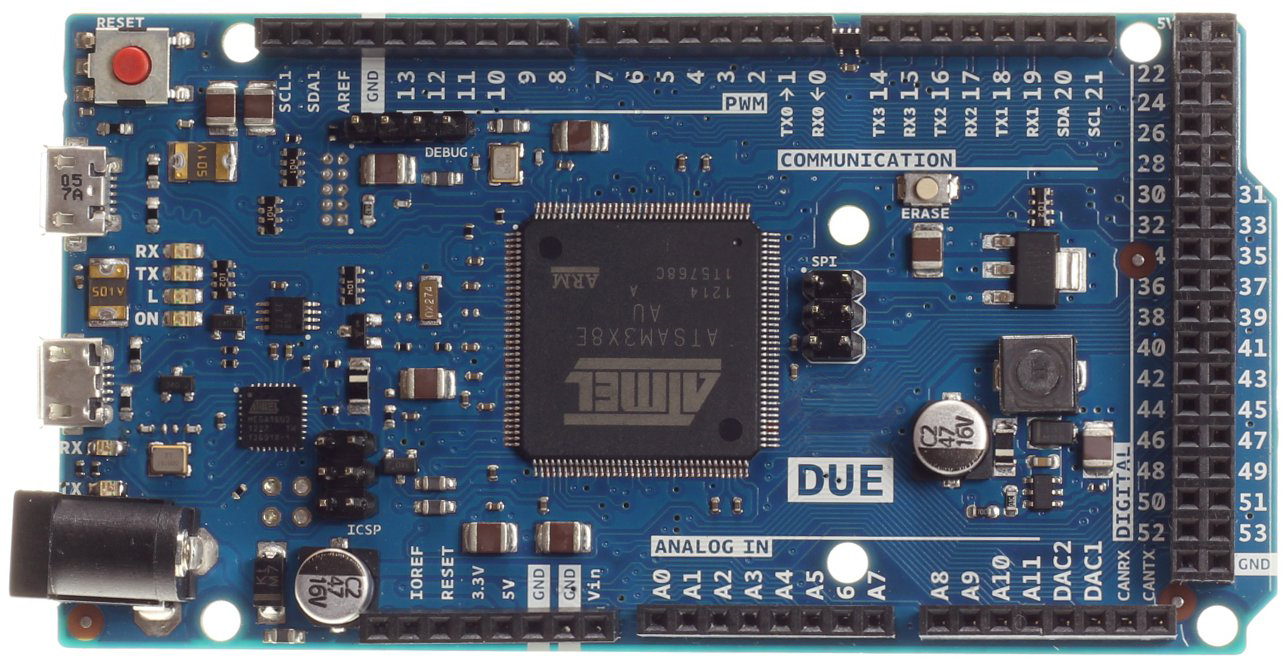
\includegraphics[scale=0.3]{due_board.jpg}
	\caption{Фотография платы.}
	\label{fig:DueBoard}
\end{figure}
\begin{table}
\centering
\begin{tabular}{|c|c|}
\hline 
Микроконтроллер & AT91SAM3X8E \\ 
\hline 
Рабочее напряжение & 3,3 В \\ 
\hline 
Входное напряжение (рекомендуемое) & 7-12 В \\ 
\hline 
Входное напряжение (предельное) & 6-20 В \\ 
\hline 
Цифровые Входы/Выходы & 54 \\ 
\hline 
Аналоговые входы & 12 \\ 
\hline 
Аналоговые выходы & 2 (ЦАП) \\ 
\hline 
Общий выходной постоянный ток & 50 мА \\ 
\hline 
Постоянный ток через вывод 3,3 В & 800 мА \\ 
\hline 
Постоянный ток через вывод 5 В & 800 мА \\ 
\hline 
Флеш-память & 512 КБ \\ 
\hline 
ОЗУ & 96 КБ(64 КБ и 32 КБ)\\ 
\hline 
Тактовая частота & 84 МГц \\ 
\hline 
\end{tabular} 
\caption{Характеристики платы.}
\label{tab:DueBoard}
\end{table}
На плате DUE V1.6 имеется 54 цифровых вход/выхода, 12 аналоговых входов, 4 UARTа (аппаратных последовательных порта), a генератор тактовой частоты 84 МГц, связь по USB с поддержкой OTG, 2 ЦАП (цифро-аналоговых преобразователя), 2 TWI, разъем питания,  разъем SPI, разъем JTAG, кнопка сброса и кнопка стирания. Так же 12 аналоговых входов, каждый из которых может обеспечить разрешение 12 бит (т.е. 4096 различных значений).

Так как эта линейка контроллеров от Elecfreaks очень популярна, DUE V1.6 выпускается большими сериями и дешевле конкурентов, кроме того, для него существует масса библиотек и сопутствующих технических решений, которые позволяют уменьшить срок выхода на рынок и повысить ремонтопригодность. Надо заметим простоту интеграции в разработку благодаря проекту ''DueVGA'' с открытым кодом на сайте распределённой системы управления версиями GitHub\cite{s_2}. Этот проект имеет уже готовую библиотеку для работы с видео интерфейсом VGA. Остановим выбор на этом контроллере.

\section{Привод}
\textit{Когда появится приложение создать ссылку на даташиты шаговых двигателей}

Привод должен не только выполнять задачу передачи вращающего момента, то так же чтобы упростить модуль позиционирования тест-объекта, имеет смысл использовать двигатель с управляемым углом поворота. Оно из лучших решений данной задачи - это шаговый двигатель. Большую часть рынка занимают гибридные 2-х/3-х/5-ти фазные шаговые двигатели. Производители заверяют, что погрешность таких двигателей не больше 5\% из-за технологических не совершенств зубцов(точек интенсивных магнитных полей к которым разворачивается ротор).
Имеем следующие параметры системы(см. табл.\ref{tab:MechParamSys})

\begin{table}[ht]
\centering
\begin{tabular}{|c|c|c|c|c|}
\hline 
Скорость передвижения каретки $V$, см/сек & 10\\
\hline 
Радиус передачи момента вращения от вала к ремню $R$, см & 0.5\\
\hline 
Вес каретки $m$, Н & 30\\
\hline 
Коэфициент усилия для передвижения каретки $\theta$ & 1.1\\
\hline 
КПД передачи $\eta$ & 0.9 \\
\hline 

\end{tabular} 
\caption{Параметры системы}
\label{tab:MechParamSys}
\end{table}
Расчет момента удержания шагового двигателя, из уравнения \ref{eq:frec}, из \ref{eq:moment} получим момент вращения вала $M=18.33$ [Н*см], на графике зависимости крутящего момента от частоты вращения для гибридных шаговых двигателей \ref{fig:MomentFrequency} видно, что при частоте $\nu=191$ крутящий момент ослабляется на 15\%, наш привод должен развивать удерживающий момент не меньше $M_{p}=18.3*1.15=21$ [Н*см]
\begin{equation}
\label{eq:frec}
\nu =\frac{V*60}{2*\pi*R}= \frac{10*60}{2*\pi*0.5}=191
\end{equation}

\begin{equation}
\label{eq:moment}
M=\frac{m*\theta*R}{\eta}= \frac{30*1.1*0.005*100}{0.9}=18.33
\end{equation}

\begin{figure}[ht]
	\centering
     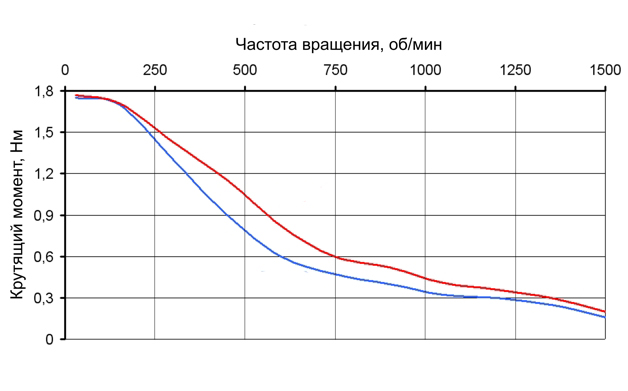
\includegraphics[scale=2.5]{moment_of_frequency_graphic.jpg}
	\caption{График зависимости крутящего момента от частоты вращения шагового двигателя.}
	\label{fig:MomentFrequency}
\end{figure}

Шаговый двигатель 17HS8401(см. рис.\ref{fig:17hs8401_step_motor}) развивает удерживающий крутящий момент $M_{p}=52$ [Н*см], минимальный угол поворота 1.8 градуса, погрешность $\xi=\frac{1.8*0.05*2*\pi*0.5}{360}=8*10^{-3} $[мм]. 17HS8401 используется в 3D принтерах и как следствие активно используется, имеет отработанные решения, готовые драйверы, это упростит встраивание в нашу проект.

\begin{figure}[ht]
	\centering
     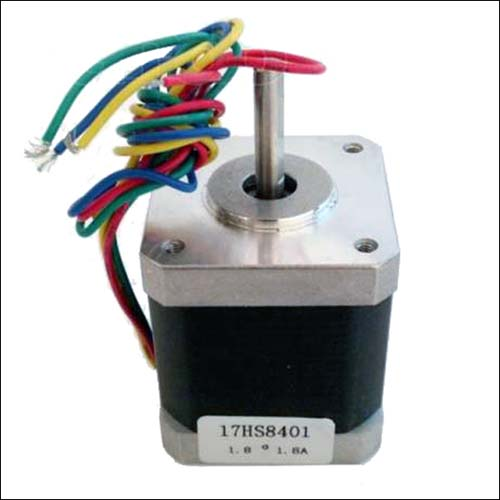
\includegraphics[scale=0.3]{17hs8401_step_motor.jpg}
	\caption{Фотография шагового двигателя.}
	\label{fig:17hs8401_step_motor}
\end{figure}
Драйвер используется для упрощения подключения шагового двигателя к контроллеру, поскольку напряжение управление не мощным шаговым двигателем обычно в диапазоне от 12 до 48 вольт, поэтому перед контроллером необходим усилительный каскад, если не использовать драйвер. Одно из готовых решений для шагового двигателя 17HS8401 - сборка MP1510 с драйвером А4988 (см. рис.\ref{fig:Step_Motor_Driver}).
\begin{figure}[h]
    \centering
    \begin{subfigure}[b]{0.45\textwidth}
    \centering
        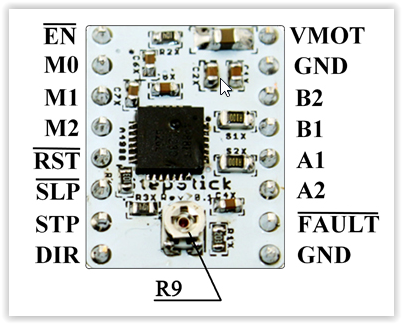
\includegraphics[scale=0.4]{Step_Motor_Driver.PNG}
        \caption{}
    \end{subfigure}
    \begin{subfigure}[b]{0.45\textwidth}
    \centering
        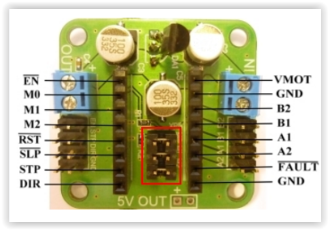
\includegraphics[scale=0.7]{Step_Motor_Driver_Uni_Model.PNG}
        \caption{}
    \end{subfigure}
    \caption{(а) Драйвер шагового двигателя А4988;
    (б) Универсальный модуль подключения драйвера ш.д. MP1510}
    \label{fig:Step_Motor_Driver}
\end{figure}
A4988 и модуль драйвера шагового двигателя(MP1510) содержат набор усилительных каскадов, которые при подачи сигнала подают напряжение в 12 вольт на вход двигателя. Контроллер управляет драйвером импульсами напряжения 5 вольт и периодом не меньше 2 мкс.

\section{Концевики}
Ограничители передвижения каретки или по другому концевики могут быть механическими, но мы остановимся на оптических(см. рис.\ref{fig:optical_end}). В их основе лежит оптрон tcst2103.
\begin{figure}[ht]
	\centering
     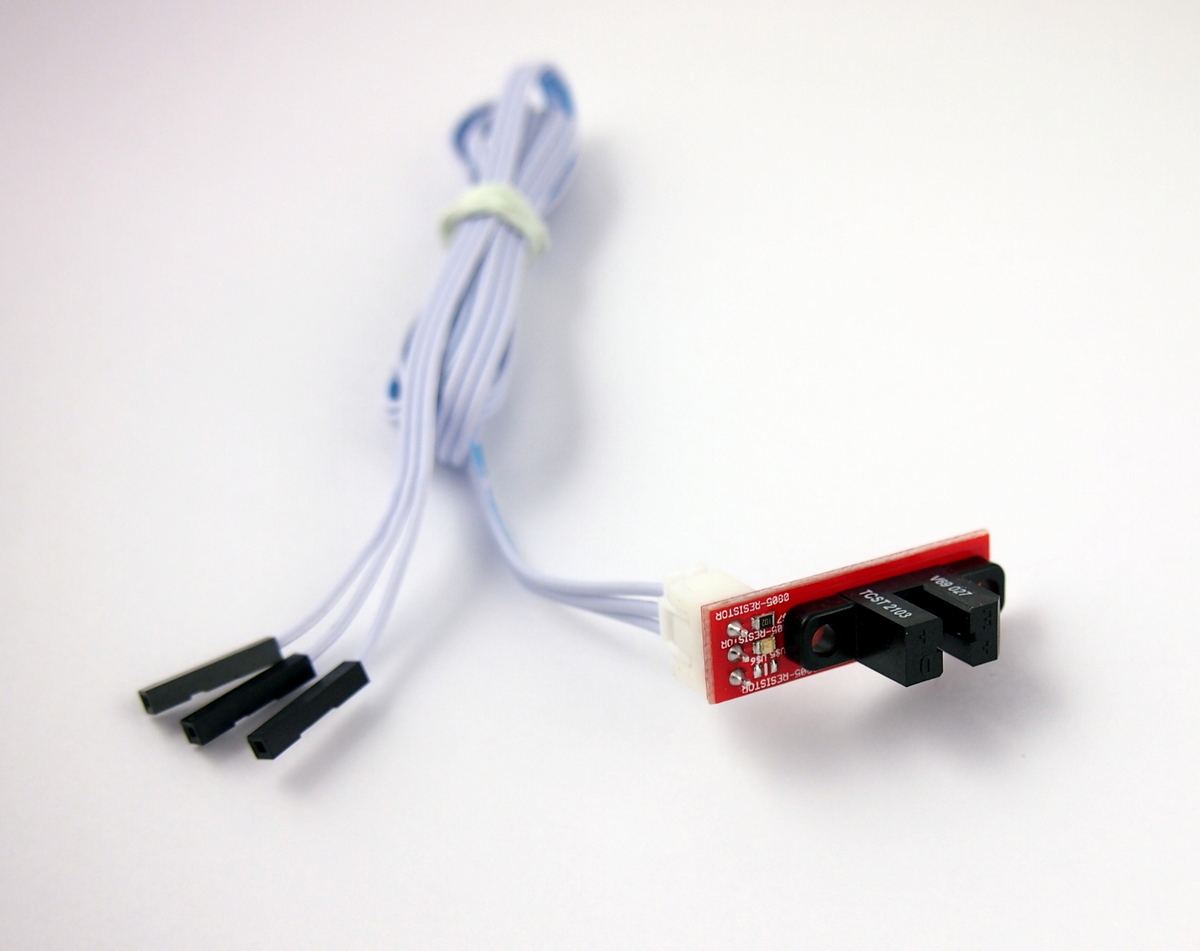
\includegraphics[scale=0.15]{optical_endswitch_with_cable_80cmP1240752.jpg}
	\caption{Оптический ограничитель передвижения каретки.}
	\label{fig:optical_end}
\end{figure}

\section{Датчики определения слайда}
\textit{Когда будет готово ТЗ проверить соответствие опорному числу 10-ти для расчета количества диапозитивов}
При помещении слайда в каретку система определяет диапозитив, его пространственную ориентацию, для этого у каждого слайда должен быть оригинальный идентификационный номер. По Т.З. количество диапозитивов больше 10-ти, а так же нужно учесть возможное увеличения их числа.
\begin{figure}[ht]
	\centering
     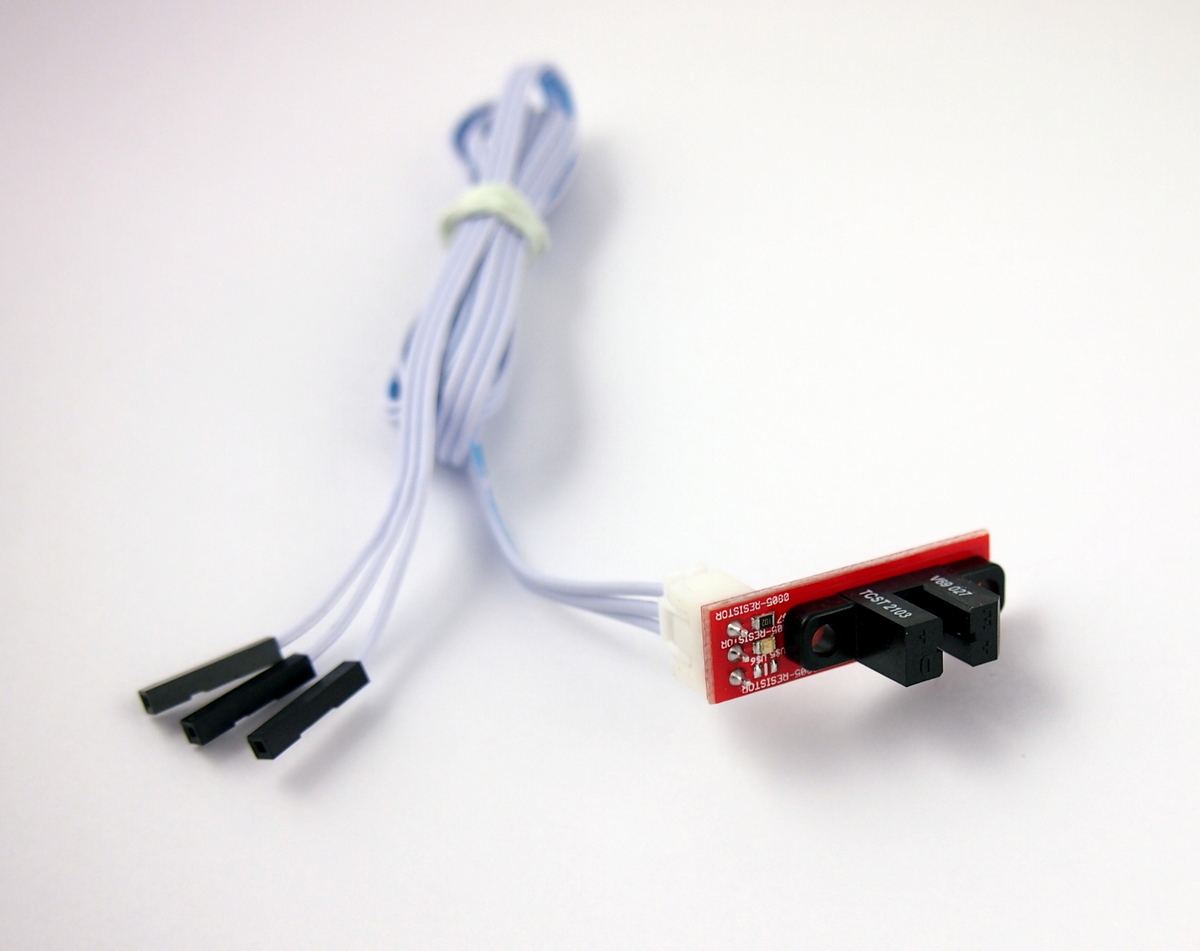
\includegraphics[scale=0.15]{optical_endswitch_with_cable_80cmP1240752.jpg}
	\caption{Оптический ограничитель передвижения каретки.}
	\label{fig:optical_end}
\end{figure}